\documentclass[tikz]{standalone}
%\usepackage{tikz}
\usetikzlibrary{intersections,backgrounds}
\title{Tikz Standalone}
\begin{document}
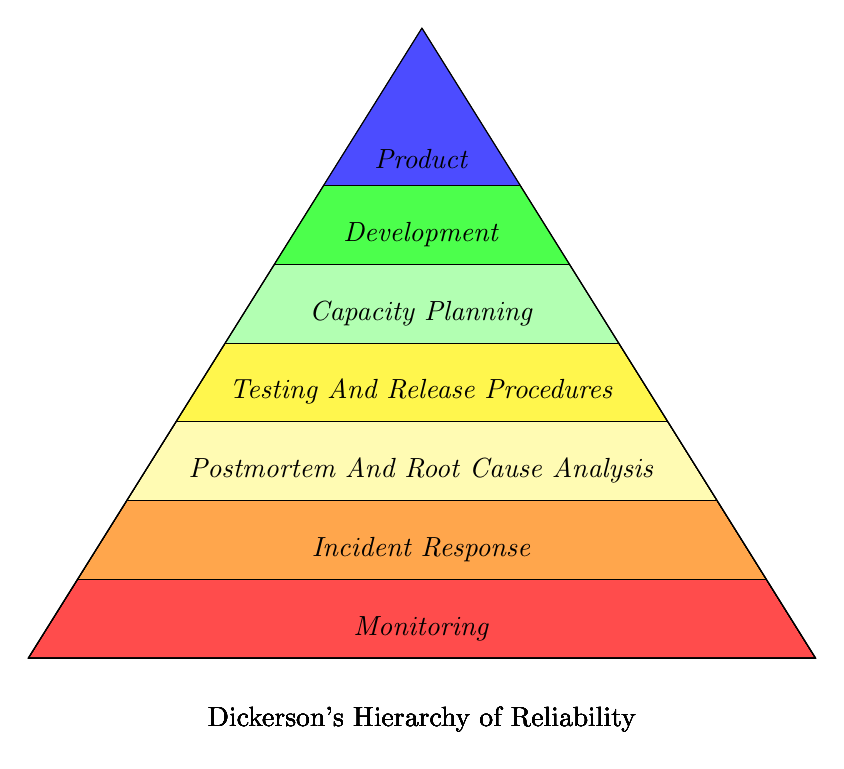
\begin{tikzpicture}
\def\colorlist{{"red!70", "orange!70", "yellow!30","yellow!70", "green!30", "green!70", "blue!70"}}
\coordinate (A) at (-5,0) {};
\coordinate (B) at ( 5,0) {};
\coordinate (C) at (0,8) {};
\draw[name path=AC] (A) -- (C);
\draw[name path=BC] (B) -- (C);
\foreach \y/\A [count=\xi starting from 0, evaluate=\y as \nexty using (\y+1, evaluate=\xi as \grad using int(\xi*15)] in {0/Monitoring ,1/Incident Response,2/Postmortem And Root Cause Analysis,3/Testing And Release Procedures,4/Capacity Planning,5/Development,6/Product} {
\pgfmathsetmacro\myfill{\colorlist[\xi]}
  \begin{scope}[on background layer]
    \clip[preaction={draw}] (-5,0) -- (5,0) -- (0,8) -- cycle;
    \fill[\myfill] (-5,\y) rectangle (5,\nexty);
    \fill[\myfill] (-5,6) rectangle (5,8);
    \end{scope}
    \path[name path=horiz,] (A|-0,\y) -- (B|-0,\y);
    \draw[name intersections={of=AC and horiz,by=P},
          name intersections={of=BC and horiz,by=Q}] (P) -- (Q)
        node[midway,above=0.1cm] {\emph{\A}};
         \node [below=0.5cm, align=flush center,text width=8cm] at (0,0)
        {
           Dickerson's Hierarchy of Reliability  
        };
}
\end{tikzpicture}
\end{document}